\clearpage
\section{Ordinalistické pojetí chování spotřebitele (princip, definice indiferenčního bodu,
indiferenční křivky a indiferenční mapy, definice a vztah pro mezní míra substituce ve
spotřebě, definice a rovnice linie rozpočtu, definice a vztah pro mezní míra substituce
ve směně, rovnováha spotřebitele, definice a vztah pro mezní míra substituce) a
odvození individuální poptávky.}

\subsection{Princip}
Spotřebitel volí mezi kombinacemi statků, porovnává užitek těchto kombinací a je schopný, které kombinace mu přinášejí stejný užitek -> indiferenční křivky.

\subsection{Indiferenční bod}
\begin{itemize}
    \item Body lhostejnosti
    \item Kombinace statků, které přinášejí stejné uspokojení
\end{itemize}

\subsection{Indiferenční křivky}
Vznikají spojením indiferenčních bodů

\subsection{Indiferenční mapy}
Souhrn indiferenčních křivek, které tvoří \uv{vrstevnice} uspokojení. Křivky na mapě se neprotínají. \\
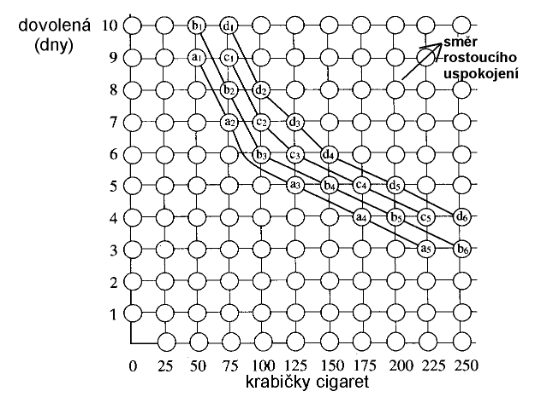
\includegraphics[width=16cm]{images/06_indif_mapa.png}

\subsection{Mezní míra substituce ve spotřebě}
\begin{itemize}
    \item Poměr, ve kterém je možno substituovat statek druhým statkem, aby užitek zůstal nezměněný.
    \item $MRS_C=|\frac{\Delta Y}{\Delta X}|$
    \item Sklon indiferenční křivky v daném bodě.
\end{itemize}
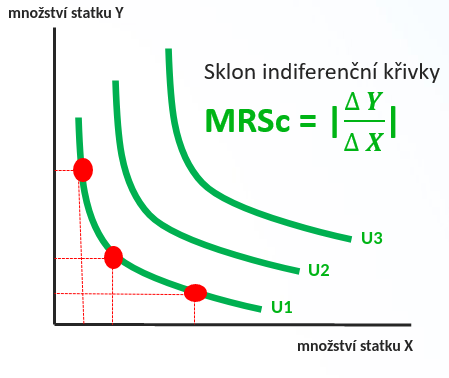
\includegraphics{images/06_mrsc.png}

\subsection{Linie rozpočtu}
\begin{itemize}
    \item Možnosti kombinací, které může spotřebitel mít při daných omezeních (výše důchodu, omezení dostupnosti)
    \item $P_X \cdot X+P_Y \cdot Y = I$, kde $I$ je důchod, $P_X$ je cena statku $X$
    a $P_Y$ je cena statku $Y$.
\end{itemize}
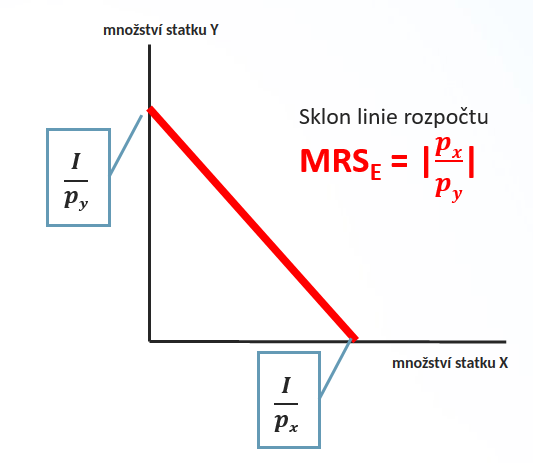
\includegraphics[width=16cm]{images/06_pr_spotr_m.png}

\subsection{Mezní míra substituce ve směně}
\begin{itemize}
    \item Poměr množství 2 statků, které lze koupit za stejný důchod.
    \item Sklon linie rozpočtu.
    \item $MRS_E=\frac{p_x}{p_y}$, kde $p$ je cena
\end{itemize}

\subsection{Rovnováha spotřebitele}
\begin{itemize}
    \item Nastává, pokud platí $MRS=MRS_E=MRS_C$, neboli $|\frac{MU_X}{MU_Y}|=|\frac{P_X}{P_Y}|=|\frac{\Delta Y}{\Delta X}|$
    \item To vlastně znamená, že hledáme místo, kde mají tyto mezní proměnné stejné hodnoty, takže místo, kde mají indiferenční křivka a linie rozpočtu stejný sklon, takže hledáme takovou indiferenční křivku, která je tečná k linii rozpočtu.
\end{itemize}

\subsection{Mezní míra substituce}
\begin{itemize}
    \item $MRS$ - \textbf{M}arginal \textbf{R}ate of \textbf{S}ubstitution
    \item poměr, v němž je možno vzájemně nahrazovat statek X a statek Y, aniž se mění celkový užitek
    \item $MRS=\frac{\Delta Y}{\Delta X}=\frac{MU_X}{MU_Y}$
\end{itemize}

\subsection{Odvození individuální poptávky}
\begin{itemize}
    \item odvozená z bodu optima, známe cenu statku (podle ní se dělají průsečíky linie rozpočtu s osami) a množství statku při této ceně
    \item Musíme zjistit, jak se změní poptávané množství statku, pokud se změní jeho cena -> nová indiferenční analýza
\end{itemize}
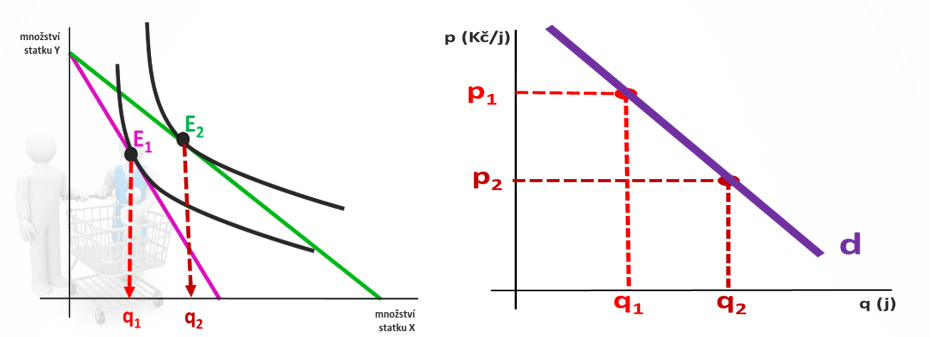
\includegraphics[width=16cm]{images/06_poptavka_indif.png}
